\documentclass{article}
\usepackage{pdfpages}
\usepackage{float}
\usepackage{enumerate}
\usepackage{amsmath}
\usepackage{amssymb}
\usepackage{graphicx}
\usepackage{url}
\usepackage{subfig}
\usepackage{color}
\usepackage{hyperref}
\usepackage[margin=0.25in]{geometry}
\hypersetup{
    colorlinks=true,
    linktoc=all
}

\title{3GC3 Final Project}
\author{Emily Horsman}
\date{December 2018}

\begin{document}

\maketitle

\begin{figure}[H]
    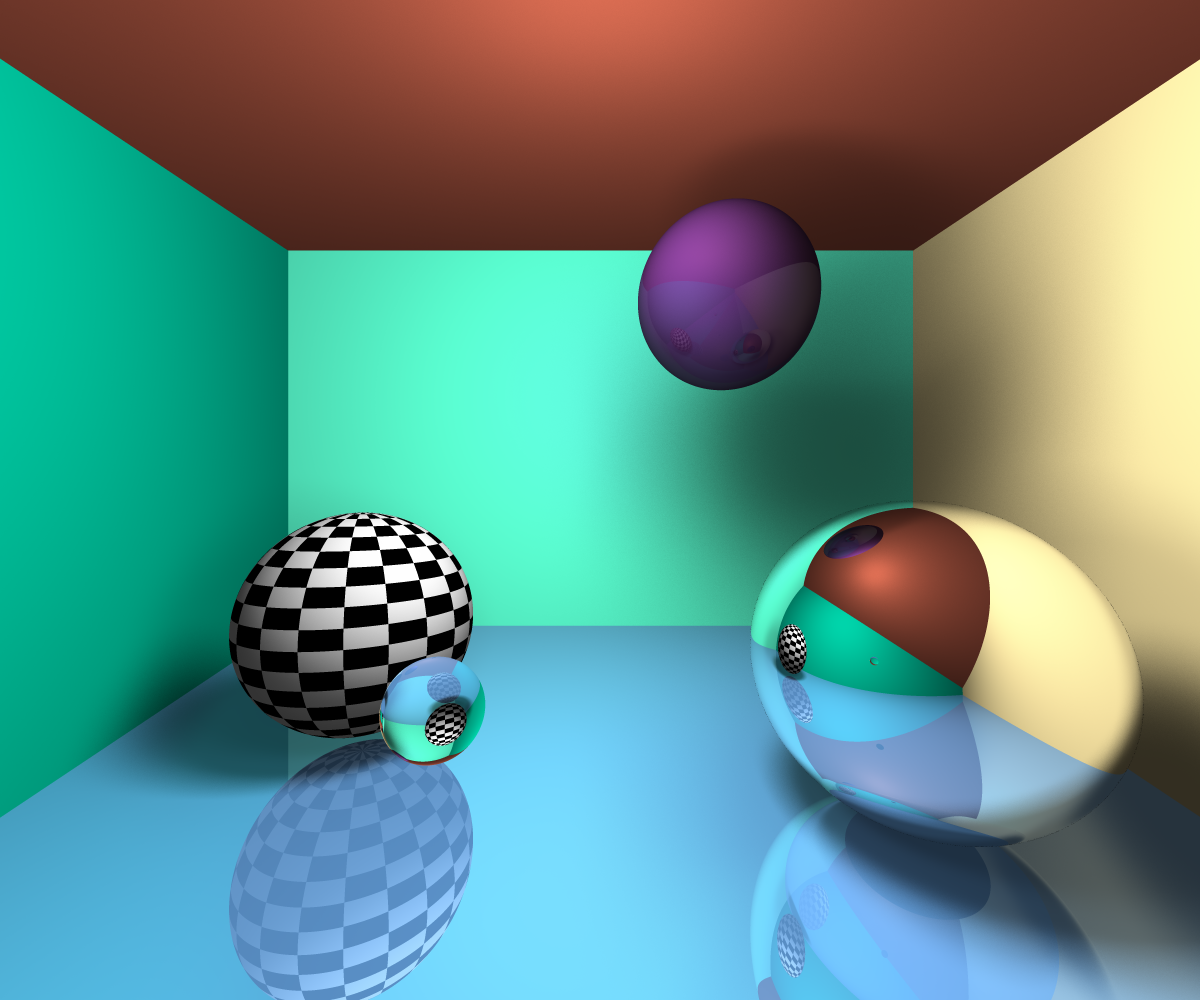
\includegraphics[width=\textwidth]{./examples/SphereRoom.png}
    \caption{Reflective floor, 100\% transparent sphere showing refraction, checkered sphere with texture mapping, mirror sphere. 64x random sampled anti-aliasing with 300 iterations for soft shadows. 13h50m of CPU time.}
\end{figure}

\newpage
\tableofcontents

\section{Scene Files}

\section{Depth of Field}

\begin{figure}[H]
    \centering
    \subfloat[\texttt{DepthOfField.scene}]{{ 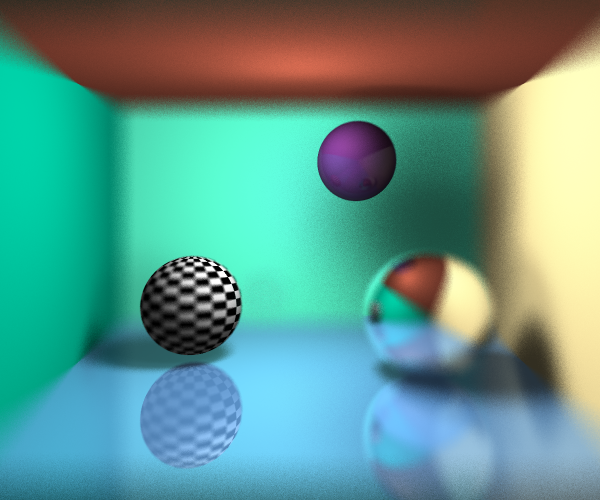
\includegraphics[width=0.45\textwidth]{./examples/DepthOfField.png} }}
    \subfloat[\texttt{DepthOfField2.scene}]{{ 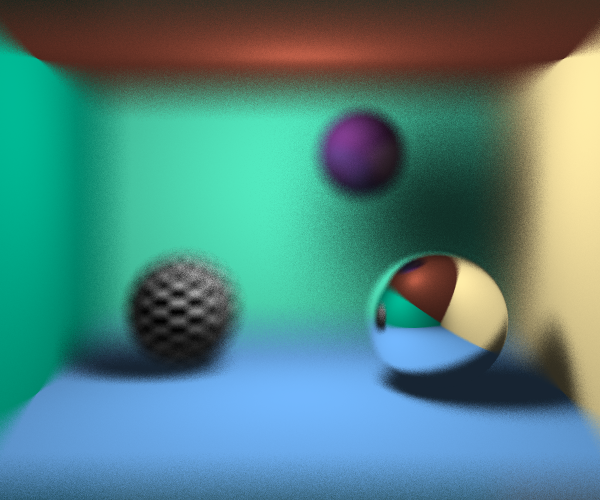
\includegraphics[width=0.45\textwidth]{./examples/DepthOfField2.png} }}
    \caption{A scene displayed with two different focal points. Minimal noise reduction, could be increased.}
\end{figure}

\section{Soft Shadows}

TODO

\section{Refraction}

\begin{figure}[H]
    \centering
    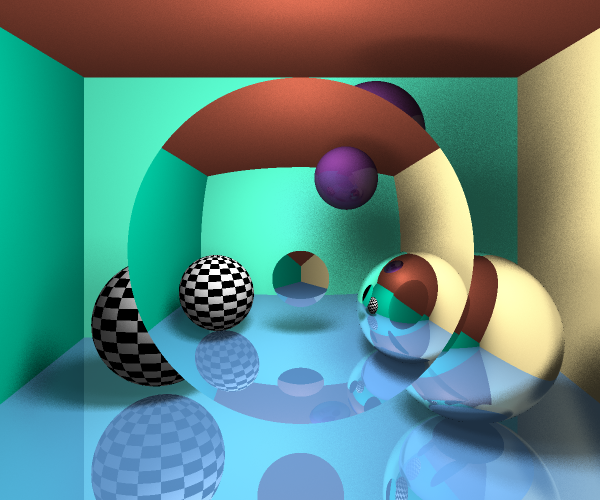
\includegraphics[width=0.6\textwidth]{./examples/DiskLens.png}
    \caption{\texttt{DiskLens.scene}. A 100\% transparent disk with a refractive index of 2.5 placed in front of the scene.}
\end{figure}

\section{Objects}

\subsection{Types}

TODO

\subsection{Texture}

TODO

\section{Anti-Aliasing}

\begin{figure}[H]
    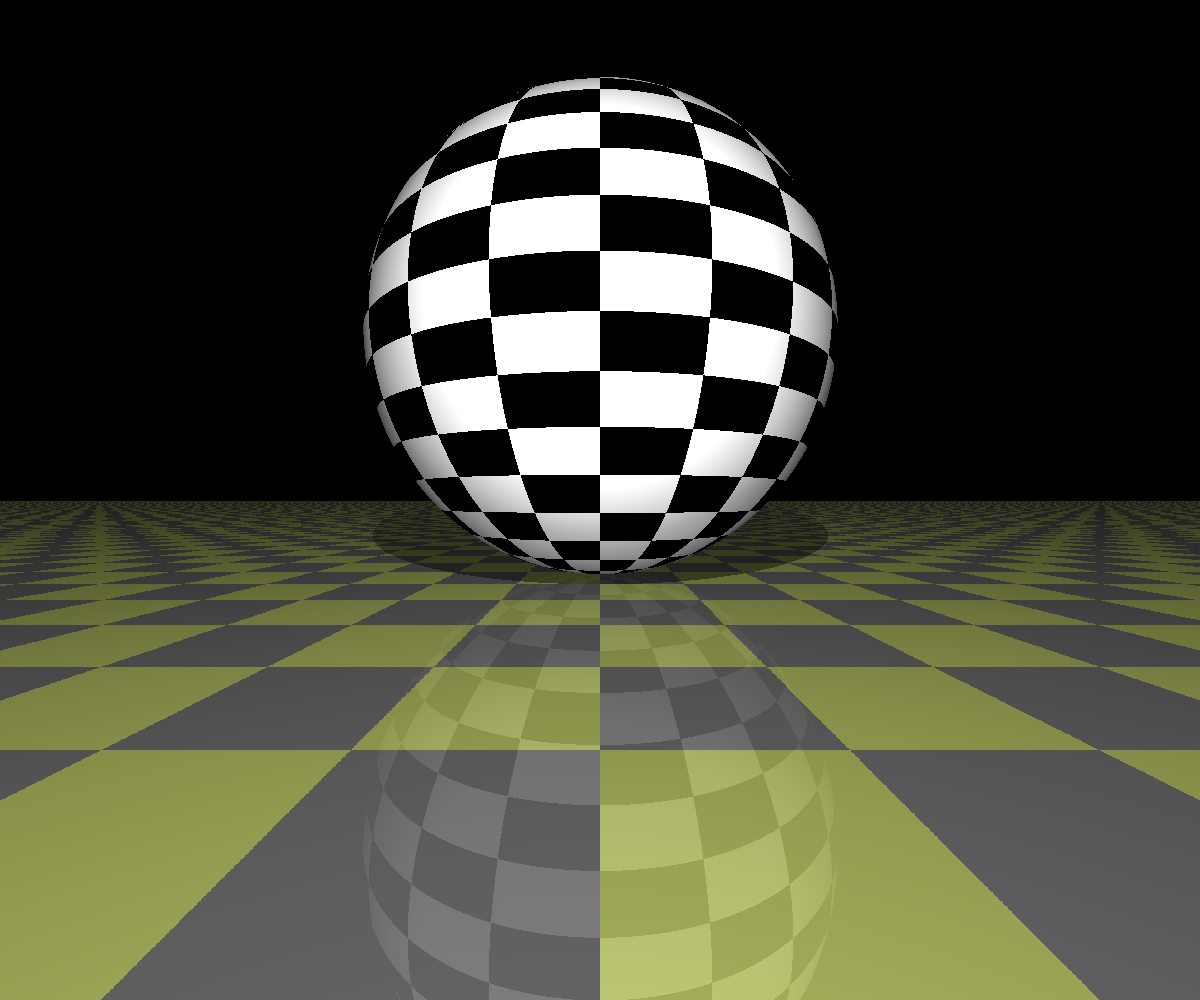
\includegraphics[width=\textwidth]{./examples/AntiAliasingComparison/Scene_noAntiAliasing.png}
    \caption{No anti-aliasing.}
\end{figure}

\begin{figure}[H]
    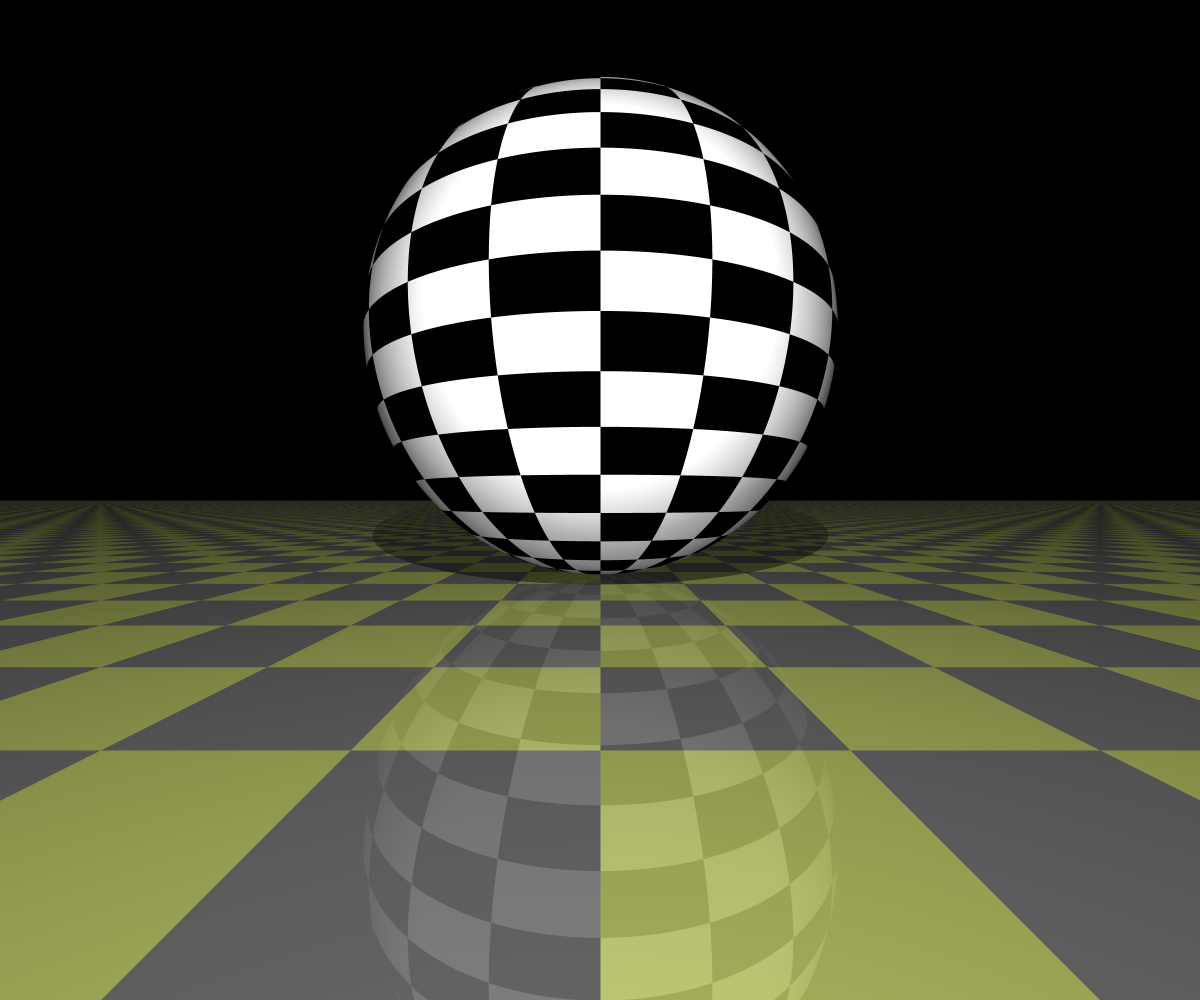
\includegraphics[width=\textwidth]{./examples/AntiAliasingComparison/Scene_regular64.png}
    \caption{64x AA using regular sampling.}
\end{figure}

\begin{figure}[H]
    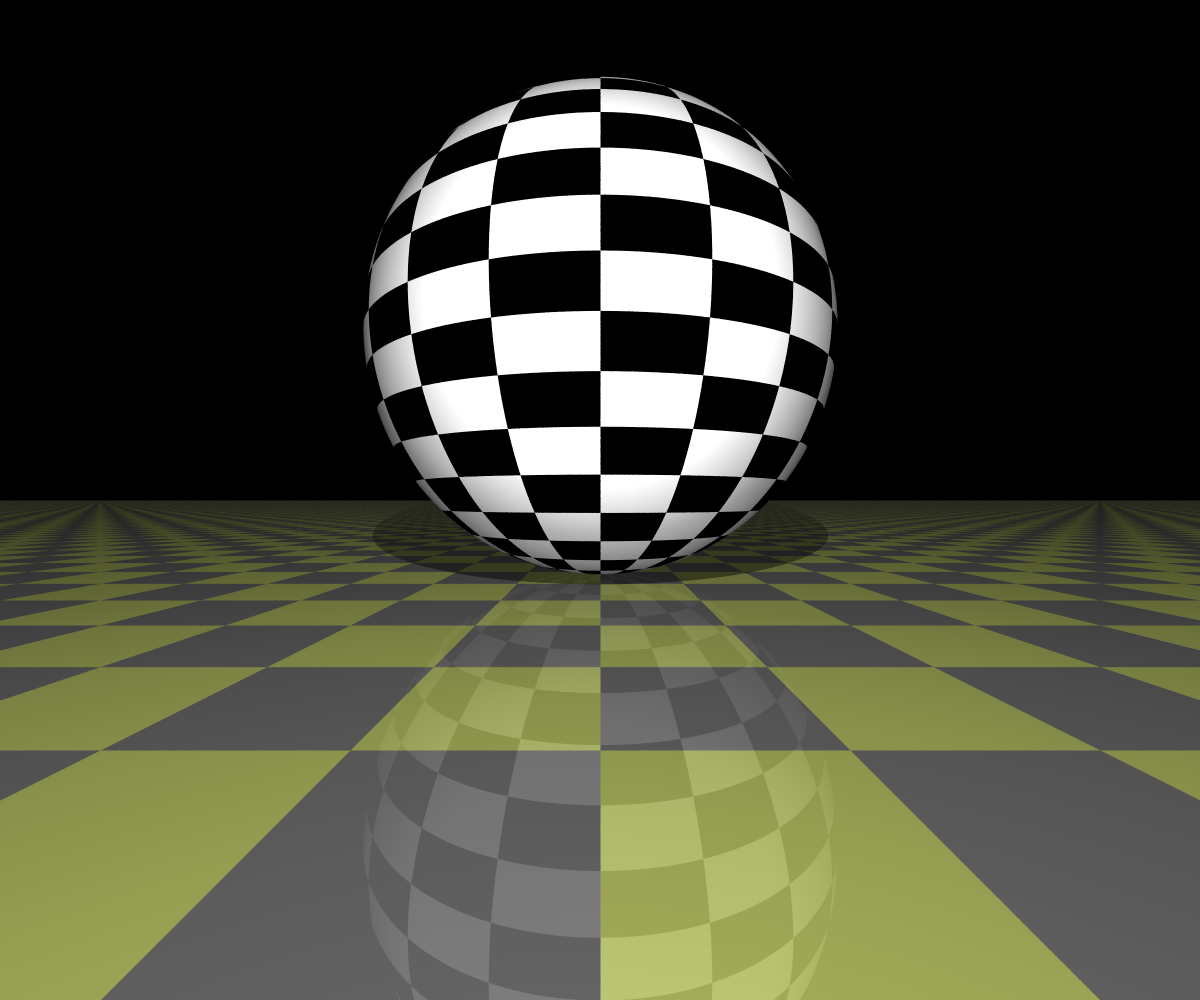
\includegraphics[width=\textwidth]{./examples/AntiAliasingComparison/Scene_random64.png}
    \caption{64x AA using random sampling.}
\end{figure}

\pagebreak

\begin{figure}[H]
    \centering
    \subfloat[Plane]{{ 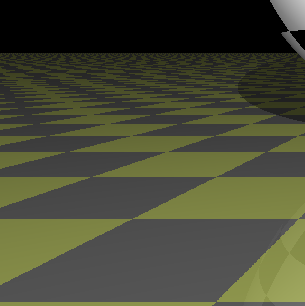
\includegraphics[width=0.3\textwidth]{./examples/AntiAliasingComparison/CheckeredPlane_noAntiAliasing.png} }}
    \subfloat[Sphere]{{ 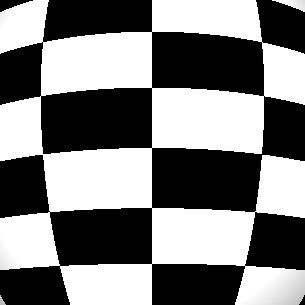
\includegraphics[width=0.3\textwidth]{./examples/AntiAliasingComparison/CheckeredSphereCrop_noAntiAliasing.png} }}
    \caption{Vanishing plane and checkered sphere without anti-aliasing.}
\end{figure}

\begin{figure}[H]
    \centering
    \subfloat[Plane]{{ 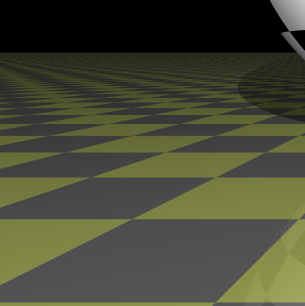
\includegraphics[width=0.3\textwidth]{./examples/AntiAliasingComparison/CheckeredPlane_regular64.png} }}
    \subfloat[Sphere]{{ 
\includegraphics[width=0.3\textwidth]{./examples/AntiAliasingComparison/CheckeredSphereCrop_regular64.png} }}
    \caption{Vanishing plane and checkered sphere with 64x AA using regular sampling.}
\end{figure}

\begin{figure}[H]
    \centering
    \subfloat[Plane]{{ 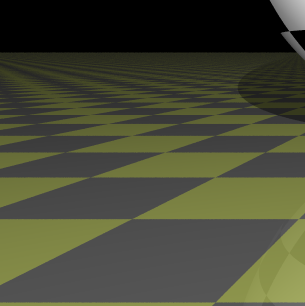
\includegraphics[width=0.3\textwidth]{./examples/AntiAliasingComparison/CheckeredPlane_random64.png} }}
    \subfloat[Sphere]{{ 
\includegraphics[width=0.3\textwidth]{./examples/AntiAliasingComparison/CheckeredSphereCrop_random64.png} }}
    \caption{Vanishing plane and checkered sphere with 64x AA using random sampling.}
\end{figure}

\section{References}

These items are referred to throughout the codebase.

\end{document}
